\documentclass[a4paper,11pt]{article}

%Package utilisé
\usepackage[latin1]{inputenc}
\usepackage[T1]{fontenc}
\usepackage[francais]{babel}
\usepackage[top=3cm, bottom=3cm, left=3cm, right=3cm]{geometry}
\usepackage{graphicx}
\usepackage{caption}
\usepackage{listings}
\usepackage{verbatim}
\usepackage{xcolor}
\usepackage{gensymb}
\usepackage{float}

\begin{document}


%Page de garde
\begin{titlepage}
    \vspace{-20px}
    \begin{tabular}{l}
	\textsc{Bannier} K\'evin
        \textsc{Loiseau} Anne-Claire
    \end{tabular}
    \hfill \vspace{10px}
\includegraphics[scale=0.1]{./images/esir.png}\\
    \vfill
    \begin{center}
        \Huge{\'Ecole sup\'erieure d'ing\'enieurs de Rennes}\\
        \vspace{1cm}
        \LARGE{3\`eme Ann\'ee}\\
        \large{Parcours IN}\\
        \vspace{0.5cm}\hrule\vspace{0.5cm}
        \LARGE{\textbf{Compte-rendu du TP n\degree 6 d'Imagerie M\'edicale}}\\
        \Large{Robotique m\'edicale : Asservissement visuel d'ultrason}
        \vspace{0.5cm}\hrule
        \vfill
        \vfill
    \end{center}
    \begin{flushleft}
        \Large{Sous l'encadrement de~:}\\
        \vspace{0.2cm}
        \large{{Alexandre} Krupa}
    \end{flushleft}
    \vfill
\end{titlepage}



\section{Objectif du TP}

L'objectif de ce TP est de simuler le positionnement automatique d'une sonde \'echographique 2D par un robot. Cela est possible en r\'ealisant un asservisemment visuel des informations denses observ\'ees dans l'image rendue par la sonde ultrasonore, et en analysant les mouvements du patient (tel que la respiration) dans le but de les compenser automatiquement.
Pour r\'ealiser cela nous allons utiliser un simulateur de sonde ultrasonore poss\'edant 6 degr\'es de libert\'e, d\'evelopp\'e par l'\'equipe Lagadic de l'INRIA. Pour arriver \`a r\'ealiser un positionnement automatique, nous allons suivre plusieurs \'etapes divis\'ees en 13 questions, et qui suivent le d\'eroulement du cours. Nous allons donc, dans ce rapport, d\'etailler ce que nous avons r\'ealis\'e \`a chacune de ces questions.


\section{Travail r\'ealis\'e}
Avant de d\'emarrer la r\'edaction du code et les r\'eponses aux questions, nous avons lanc\'es l'outil de simulation r\'ealis\'e par l'\'equipe de l'INRIA. Cet outil ouvre plusieus fen\^etres qui sont les suivantes :
\begin{itemize}
\item L'image actualis\'e de l'ultrason. Rien n'est encore cod\'e, cette image reste donc immobile.
\item L'image d\'esir\'e. Cette image n'est pas cens\'e bouger par la suite, elle montre la zone d'int\'er\^et s\'el\'ectionn\'e.
\item L'image diff\'erence entre les deux pr\'ec\'edentes. Pour le moment cela renvoit une image grise car elles sont identiques.
\item Courbe de vitesse de d\'eplacement de la sonde (translation et rotation)
\item Courbe d'erreur de position de la sonde (translation et rotation
\item Courbe d'erreur de la fonction de co\^ut
\end{itemize}

\subsection{Question 1}
Dans cette partie, nous allons appliquer les 6 degr\'es de libert\'e de la sonde, dans le but de simuler les mouvements du patient. Voici le code qui nous permet de r\'ealiser cela :
\begin{verbatim}
double ampliture_t = 0.020;
double ampliture_r = 20.0;

object_velocity[0] = ampliture_t*sin(2*M_PI*(1.0/5.0)*time);
object_velocity[1] = ampliture_t*sin(2*M_PI*(1.0/5.0)*time);
object_velocity[2] = ampliture_t*sin(2*M_PI*(1.0/5.0)*time);

object_velocity[3] = vpMath::rad(ampliture_r) * sin( 2*M_PI*(1.0/5.0)*time);
object_velocity[4] = vpMath::rad(ampliture_r) * sin( 2*M_PI*(1.0/5.0)*time);
object_velocity[5] = vpMath::rad(ampliture_r) * sin( 2*M_PI*(1.0/5.0)*time);
\end{verbatim}

%TODO Commenter le code si nécessaire

Le r\'esultat que nous obtenons s'applique directement sur l'image actualis\'e de l'ultrason, ce qui modifie \'egalement l'image de diff\'erence, et la courbe d'erreur de pose de la sonde. Voici ce que nous observons :
\begin{figure}
	\centering
		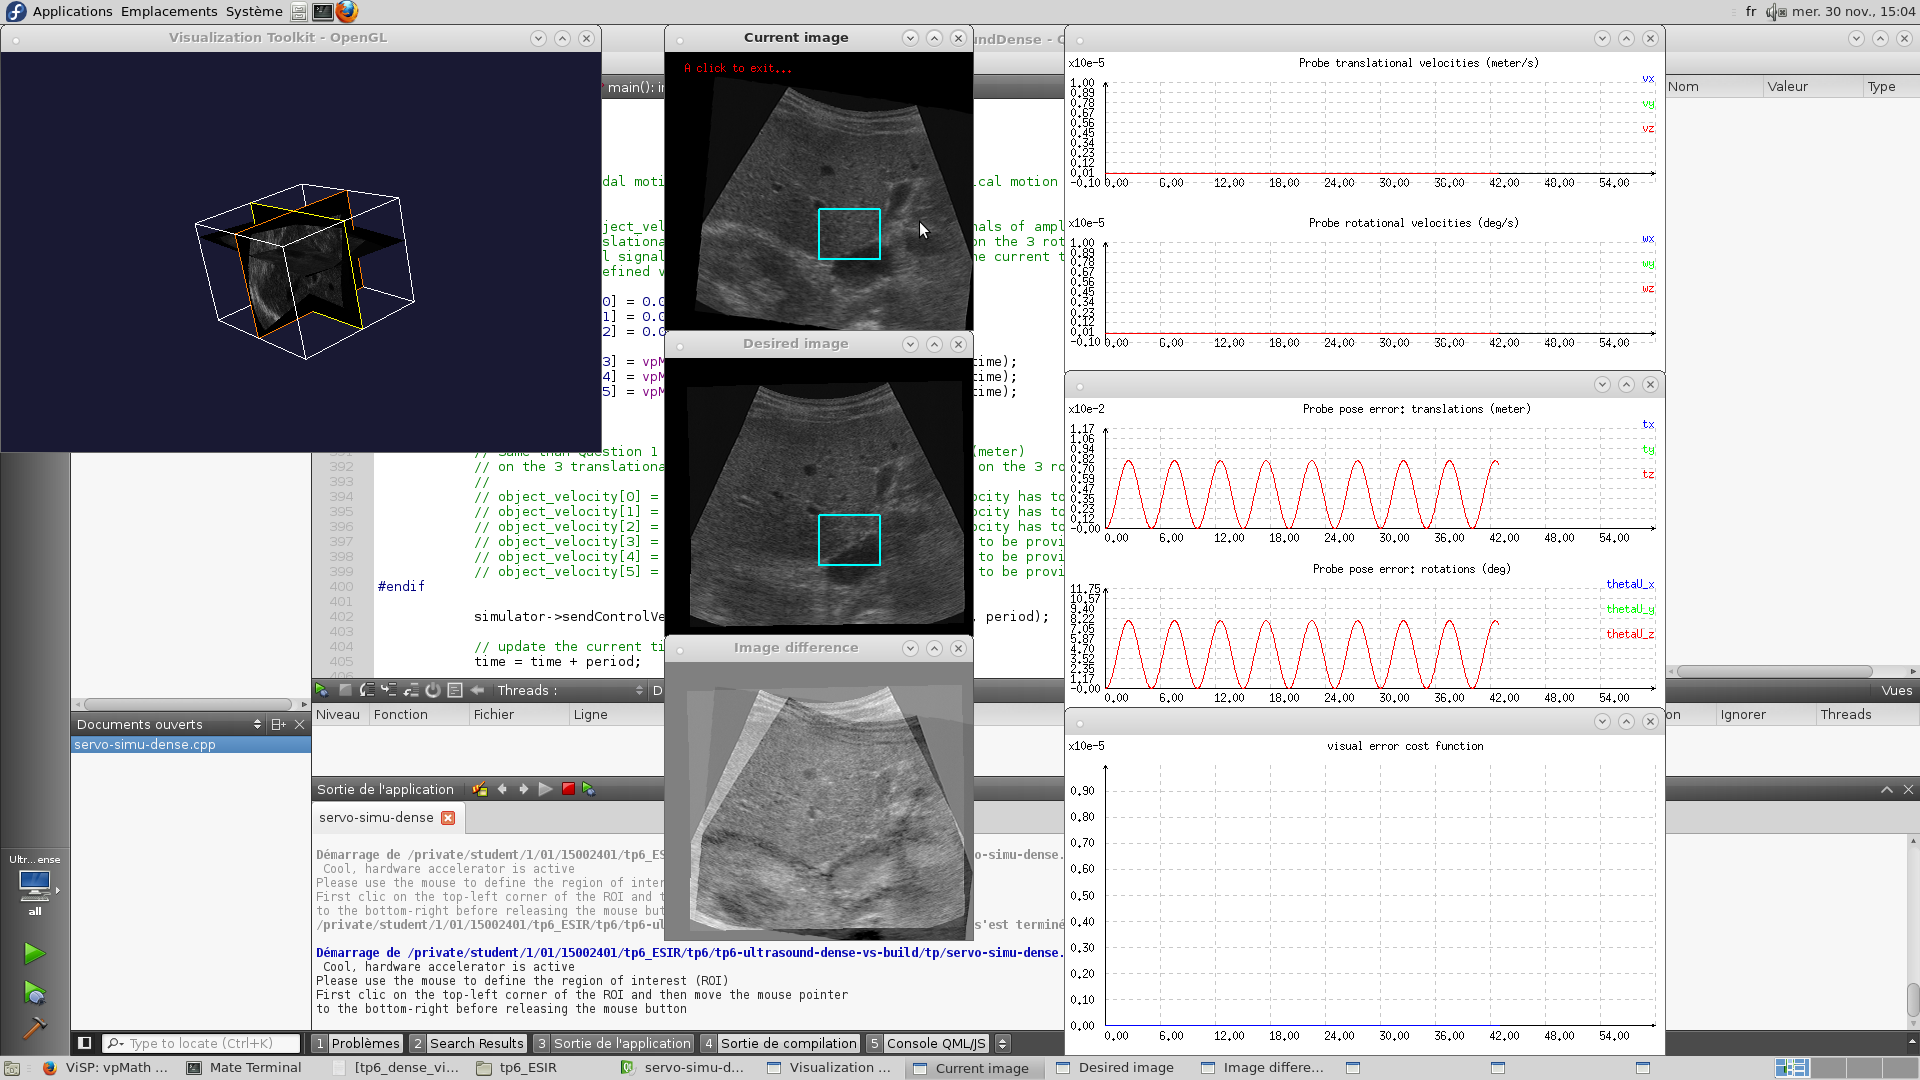
\includegraphics[width=500px]{./images/question1.png}
	\caption{Observation des mouvements simul\'e du patient}
	\label{mvtPatient}
\end{figure}

La Figure \ref{mvtPatient} montre l'\'etat du patient \`a un instant t. En effet, les mouvements sont continues, ce que nous montre bien la courbe. Nous observons sur cette Figure \ref{mvtPatient} une diff\'erence assez \'elev\'e entre l'image actuel du mouvement du patient, et l'image d\'esir\'ee, soit celle initiale. Cela est normal, car aucune compensation automatique n'est r\'ealis\'e pour le moment, il y a seulement le battement de coeur qui est simul\'e. Ce battement de coeur simul\'e par ailleurs n'est pas vraiment r\'ealiste car sa mani\'ere de bouger est r\'ealis\'e par des sinus, ce qui donne un r\'esultat tr\`es peu r\'ealiste. De plus nous obtenons une erreur identique entre la rotation et la translation, mais cela est normal puisque rien n'est compens\'e ou m\^eme appris.
Dans cette simulation, la zone d'int\'er\^et a peu d'importance puisque nous l'avons dit, aucun mouvement n'est actuellement compens\'e en fonction de cette zone, seulement la simualtion des battements du coeur est effectu\'e.

\subsection{Question 2}
%TODO Expliquer le but de la question
\begin{verbatim}
for(int i=0; i<ROI_height; i++) {
    for(int j=0; j<ROI_width; j++) {
        DesiredFeatures[i*ROI_width+j] = simulator->Image(i+Hmin, j+Wmin);
}
\end{verbatim}
%TODO Commenter le code si nécessaire

\subsection{Question 3}
%TODO Expliquer le but de la question
\begin{verbatim}
vpMatrix patchX(3,3);
patchX[0][0] = -1;  patchX[1][0] = -2;  patchX[2][0] = -1;
patchX[0][1] = 0;   patchX[1][1] = 0;   patchX[2][1] = 0;
patchX[0][2] = 1;   patchX[1][2] = 2;   patchX[2][2] = 1;

vpMatrix patchY = patchX.transpose();

vpMatrix patchZ(3,3);
patchZ[0][0] = 1;  patchZ[1][0] = 2;  patchZ[2][0] = 1;
patchZ[0][1] = 2;   patchZ[1][1] = 4;   patchZ[2][1] = 2;
patchZ[0][2] = 1;   patchZ[1][2] = 2;   patchZ[2][2] = 1;

for(int i=Hmin; i<Hmax; i++) {
	for(int j=Wmin; j<Wmax; j++) {
    	double img0Fx = ApplyPatch(2*patchX, img0, i, j);
    	double img0Fy = ApplyPatch(2*patchY, img0, i, j);
    	double img0Fz = 0;

    	double imgaFx = ApplyPatch(patchX, imga, i, j);
    	double imgaFy = ApplyPatch(patchY, imga, i, j);
    	double imgaFz = ApplyPatch(-patchZ, imga, i, j);
	
    	double imgbFx = ApplyPatch(patchX, imgb, i, j);
    	double imgbFy = ApplyPatch(patchY, imgb, i, j);
    	double imgbFz = ApplyPatch(patchZ, imgb, i, j);

        dIdx[i][j] = img0Fx + imgaFx +  imgbFx;
        dIdy[i][j] = img0Fy + imgaFy +  imgbFy;
        dIdz[i][j] = img0Fz + imgaFz +  imgbFz;
    }
}
\end{verbatim}

%TODO : Commenter l'utilisation d'une nouvelle fonction ApplyPatch

\begin{verbatim}
/**
 * @brief usImageGradient::ApplyPatch This method apply a patch to a point (i, j) in a image img
 * @param patch : the patch to apply (ex : a 3x3 image)
 * @param img : the original image
 * @param i : coordonate i of the point
 * @param j : coordonate j of the point
 * @return the result of the patch applying to this point
 */
double usImageGradient::ApplyPatch(const vpMatrix &patch, vpImage<unsigned char> &img, int & i, int & j)
{
    double result = 0;

    for(int iPatch = -(int)(patch.getRows()/2); iPatch <= (int)patch.getRows()/2; iPatch++) {
        for(int jPatch = -(int)(patch.getCols()/2); jPatch <= (int)patch.getCols()/2; jPatch++) {
            result += patch[iPatch+patch.getRows()/2][jPatch+patch.getCols()/2] * img[i+iPatch][j+jPatch];
        }
    }
    return result;
}
\end{verbatim}
%TODO Commenter le code si nécessaire

\subsection{Question 4}
%TODO Expliquer le but de la question
\begin{verbatim}
int k=0;
for(int i=0;i<ROIH; i++) {
	for(int j=0; j<ROIW; j++) {
		Ls[k][0] = dIdx[Hmin + i ][ Wmin + j];
        Ls[k][1] = dIdy[Hmin + i ][ Wmin + j];
        Ls[k][2] = dIdz[Hmin + i ][ Wmin + j];

        double x = sx*((Wmin + j)-(imgW/2));
        double y = sy*((Hmin + i)-(imgH/2));

        Ls[k][3] = y*Ls[k][2];
        Ls[k][4] = -x*Ls[k][2];
        Ls[k][5] = x*Ls[k][1] - y*Ls[k][0];
        k++;
	}
}
\end{verbatim}
%TODO Commenter le code si nécessaire

\subsection{Question 5}
%TODO Expliquer le but de la question
\begin{verbatim}
for(int i=0; i<ROI_height; i++) {
	for(int j=0; j<ROI_width; j++) {
		CurrentFeatures[i*ROI_width+j] = simulator->Image(i+Hmin, j+Wmin);
	}
}
\end{verbatim}
%TODO Commenter le code si nécessaire

\subsection{Question 6}
%TODO Expliquer le but de la question
\begin{verbatim}
double lambda = 0.1;
vpColVector VisualFeatureError;
VisualFeatureError = CurrentFeatures - DesiredFeatures; // Compute the visual feature error
probe_velocity = -lambda*Ls.pseudoInverse()*VisualFeatureError; // Compute the probe velocity
\end{verbatim}
%TODO Commenter le code si nécessaire

\subsection{Question 7}
%TODO Expliquer le but de la question
\begin{verbatim}
cost = VisualFeatureError.euclideanNorm() / nbPx;
\end{verbatim}
%TODO Commenter le code si nécessaire

\subsection{Question 8}
Avec un lambda = 0.4, l'asservissement visuel fonctionne. A chaque instant (it\'eration de la boucle), la cam\'era se re-positionne pour suivre le mouvement de l'objet. L'erreur ne d\'epasse jamais 0.02, ce qui est tr\`es performant (Figure \ref{assertVisu}). Cela se voit dans la fen\^etre 'Image Difference' : les erreurs sont tr\`es faibles et \`a peine visibles. L'erreur (affich\'ee en bas \`a droite de la Figure \ref{assertVisu}) varie en fonction des oscillations de l'objet. Plus le mouvement est rapide, plus l'erreur augmente.
\begin{figure}[H]
    \centering
    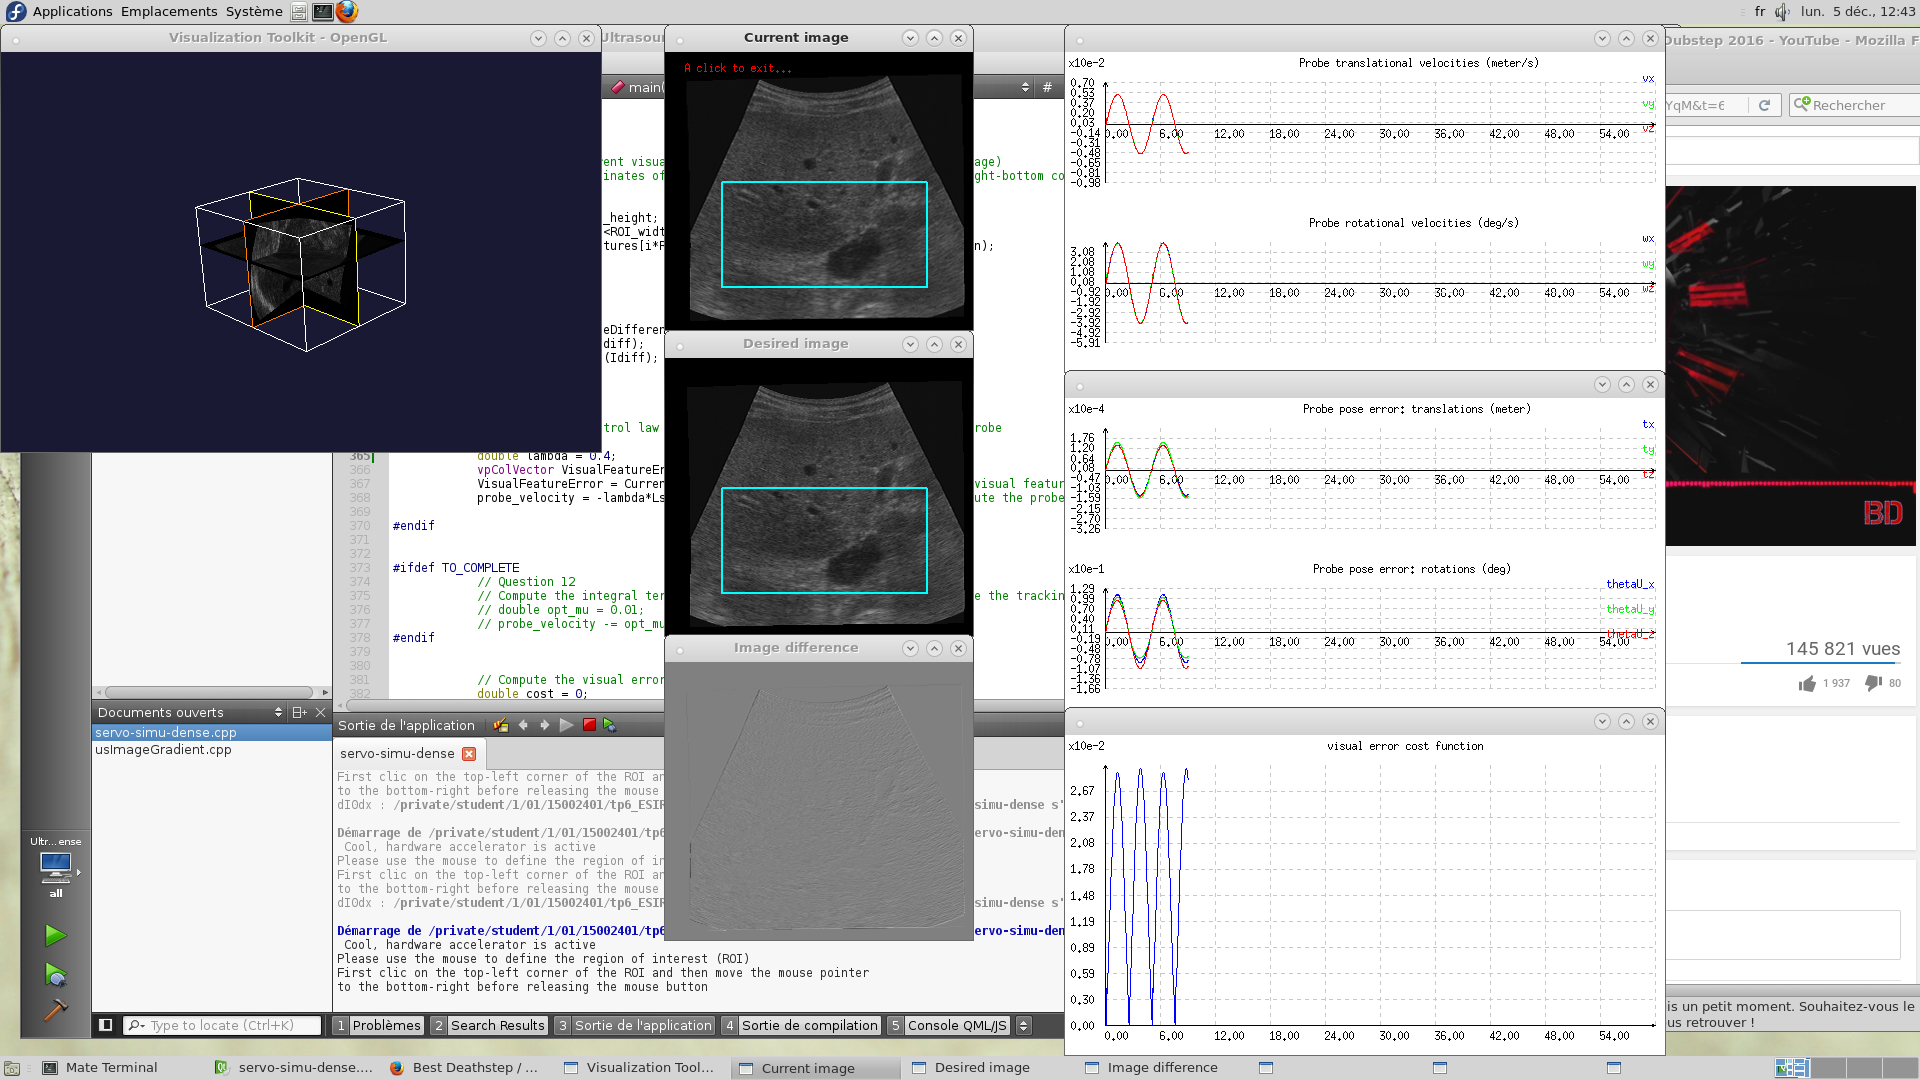
\includegraphics[width=1.0\textwidth]{./images/q8.png}
    \caption{Asservissement visuel}
    \label{assertVisu}
\end{figure}


\subsection{Question 9}
La region d'interet a beaucoup d'importance. Elle permet d'effectuer l'asservissement visuel correctement (ou non). Lorsque le ROI est grand, la loi de commande a peu de chance de se tromper de direction, parce le nombre de donn\'ees est tr\`es \'elev\'e. La minimisation de l'erreur fonctionne donc tr\`es bien (Figure \ref{largeRoi}). D\`es lors que le roi est r\'eduit, les pics de l'erreur sont plus \'elev\'es : 5.5x10-2 avec un ROI moyen contre 1.8x10-2 avec un grand ROI (figure \ref{mediumRoi}).
\par
Dans la m\^eme lign\'ee, l'erreur devient tr\`es forte lorsque le ROI est tr\`es petit (Figure \ref{smallRoi}). De plus, on constate m\^eme que dans ce cas l\`a, l'asservissement est imparfait : ça tremble. La r\'egion d'int\'er\^et \'etant tr\`es petite, les donn\'ees utiles pour l'asservissement sont pr\'esentes en petite quantit\'e, ce qui limite la pr\'ecision. Une r\'egion d'int\'er\^et de taille correcte est donc importante.

\begin{figure}[H]
    \centering
    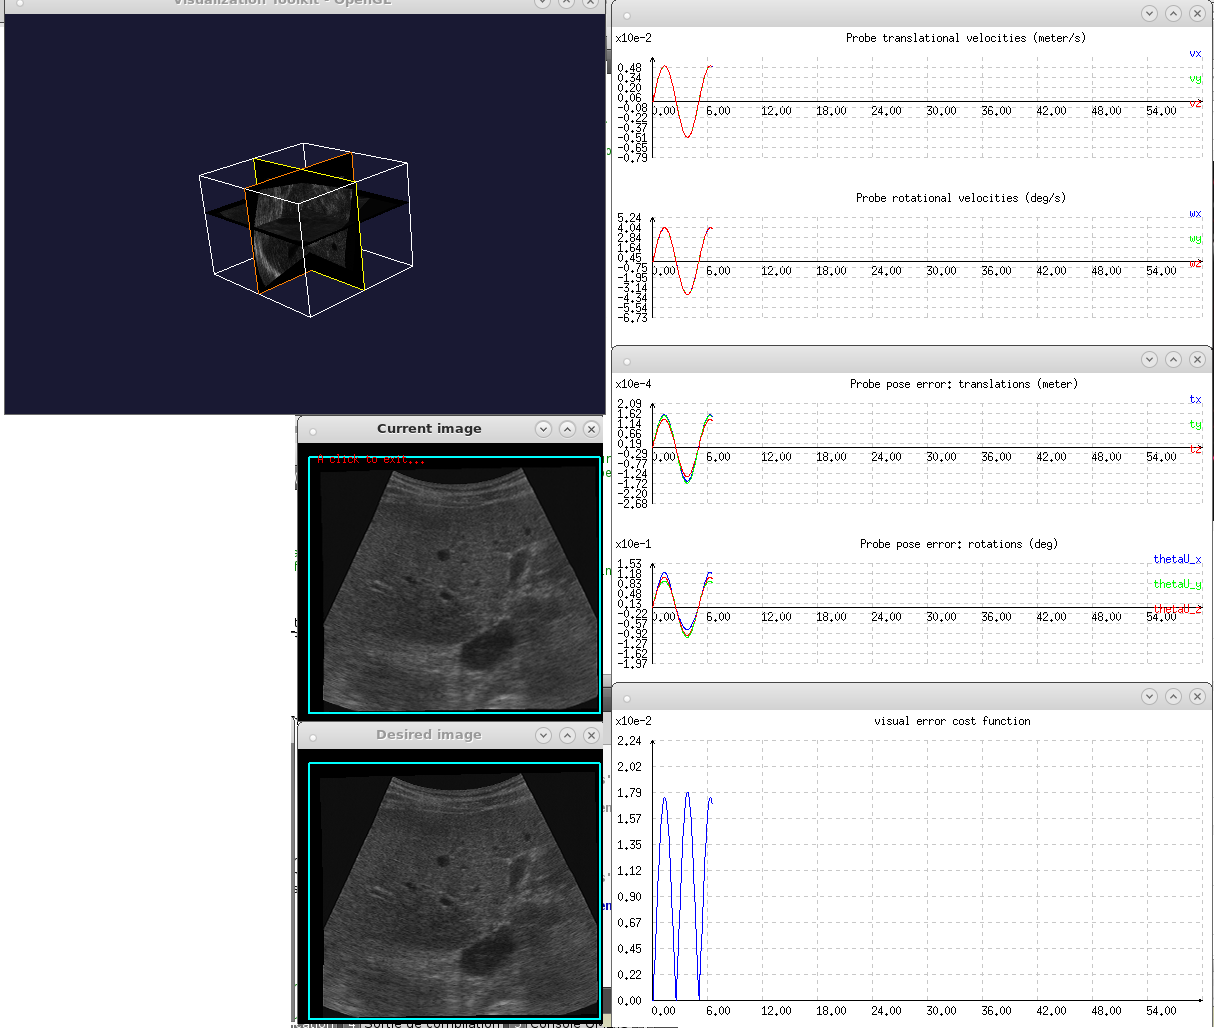
\includegraphics[width=0.5\textheight]{./images/q9_large.png}
    \caption{Asservissement avec un grand ROI}
    \label{largeRoi}
\end{figure}
\begin{figure}[H]
    \centering
    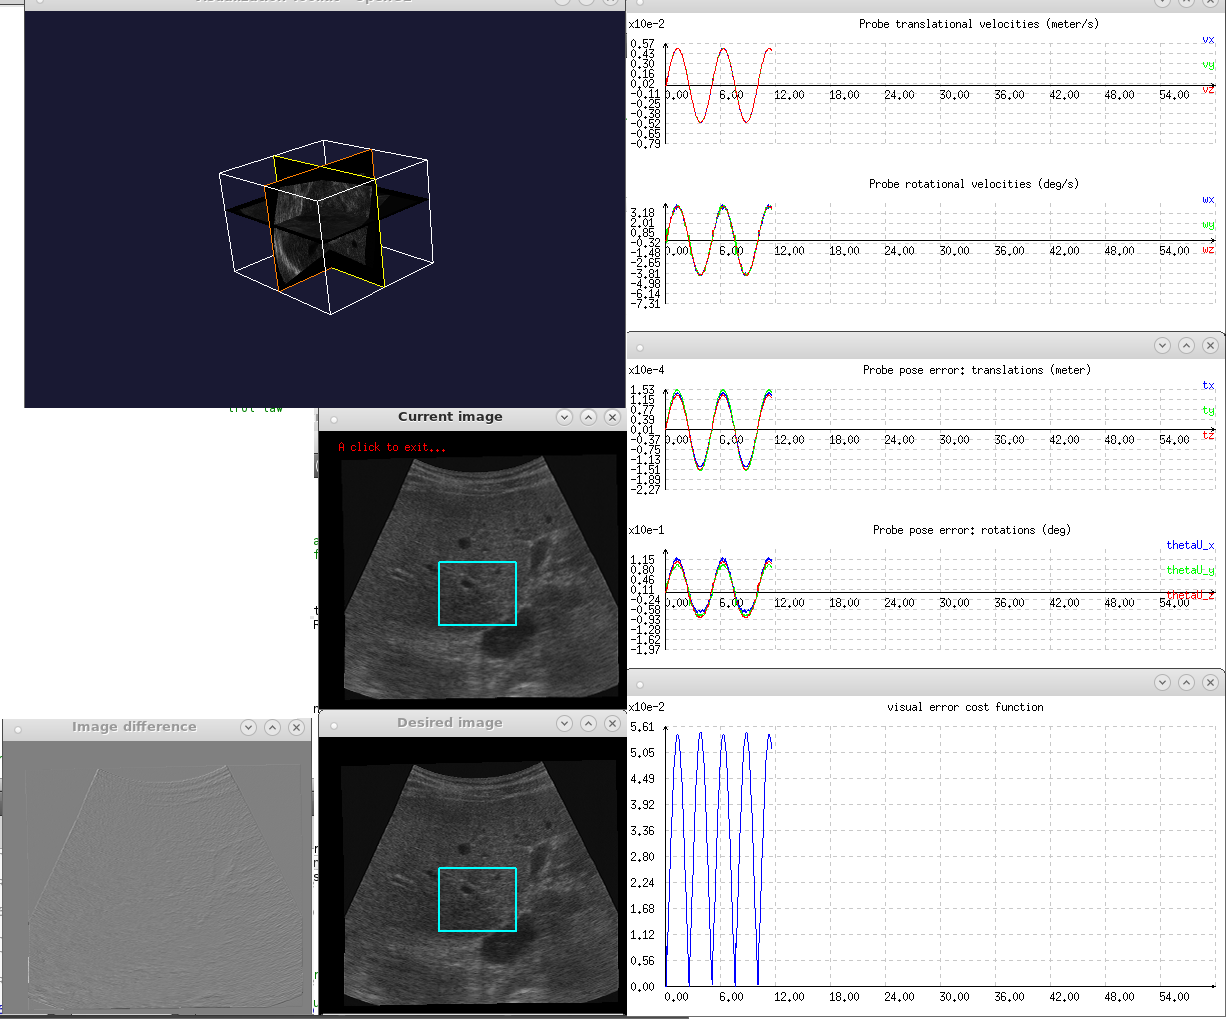
\includegraphics[width=0.5\textheight]{./images/q9_medium.png}
    \caption{Asservissement avec un ROI moyen}
    \label{mediumRoi}
\end{figure}
\begin{figure}[H]
    \centering
    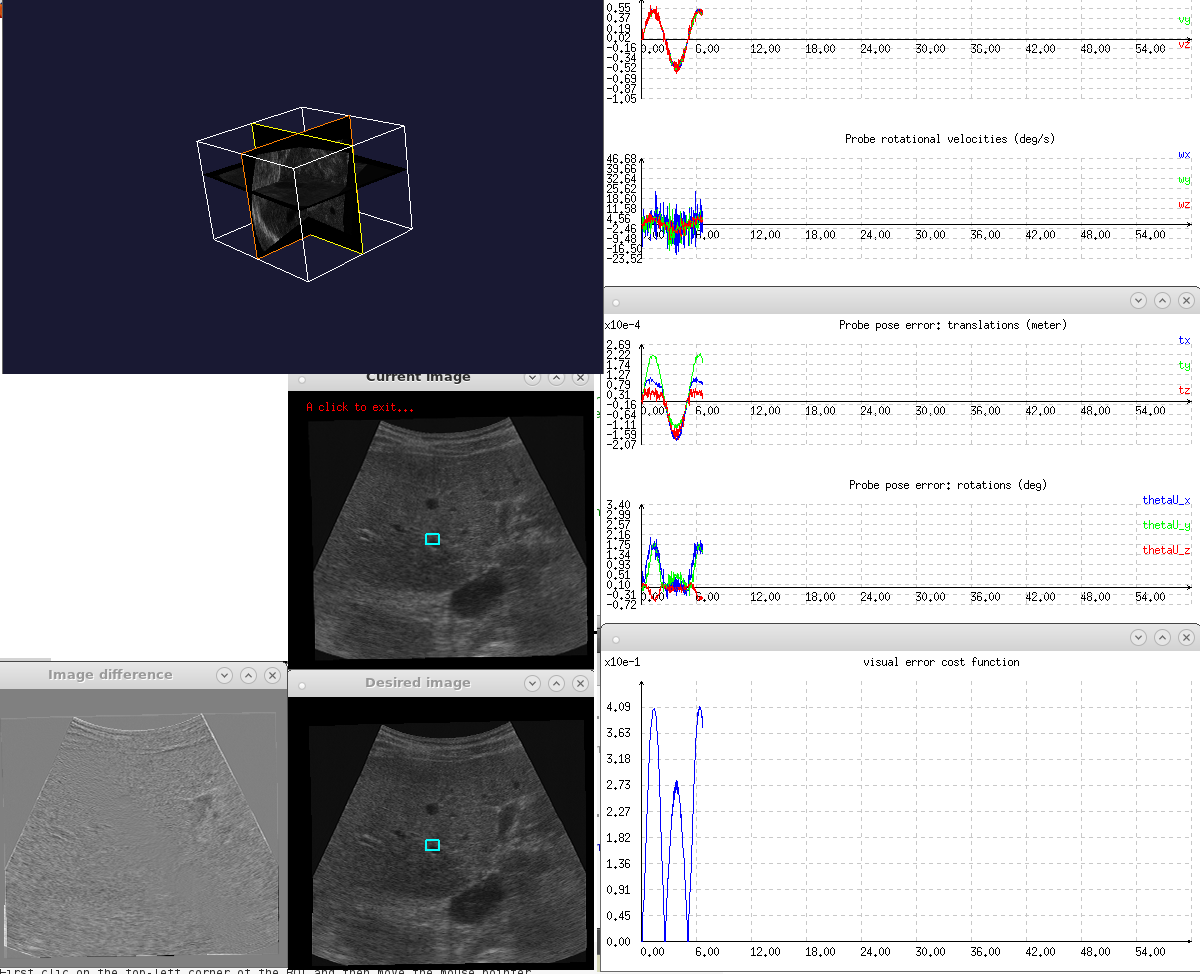
\includegraphics[width=0.5\textheight]{./images/q9_small.png}
    \caption{Asservissement avec un petit ROI}
    \label{smallRoi}
\end{figure}

\subsection{Question 10}
%TODO
\begin{figure}[H]
    \centering
    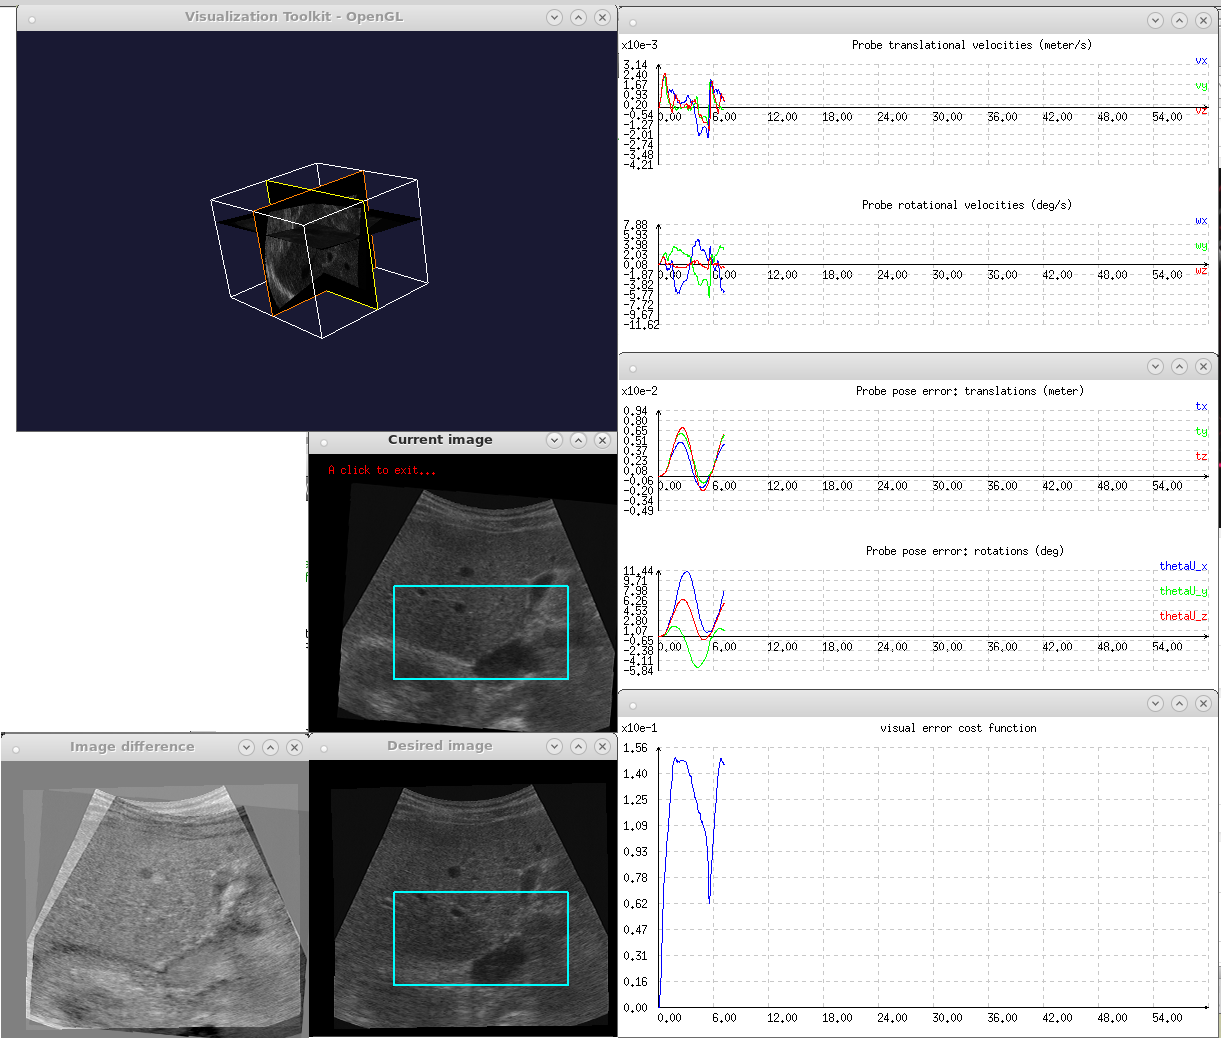
\includegraphics[width=1.0\textwidth]{./images/q10_small.png}
    \caption{Asservissement avec un petit gain (lambda=0.1)}
    \label{smallGain}
\end{figure}

\begin{figure}[H]
    \centering
    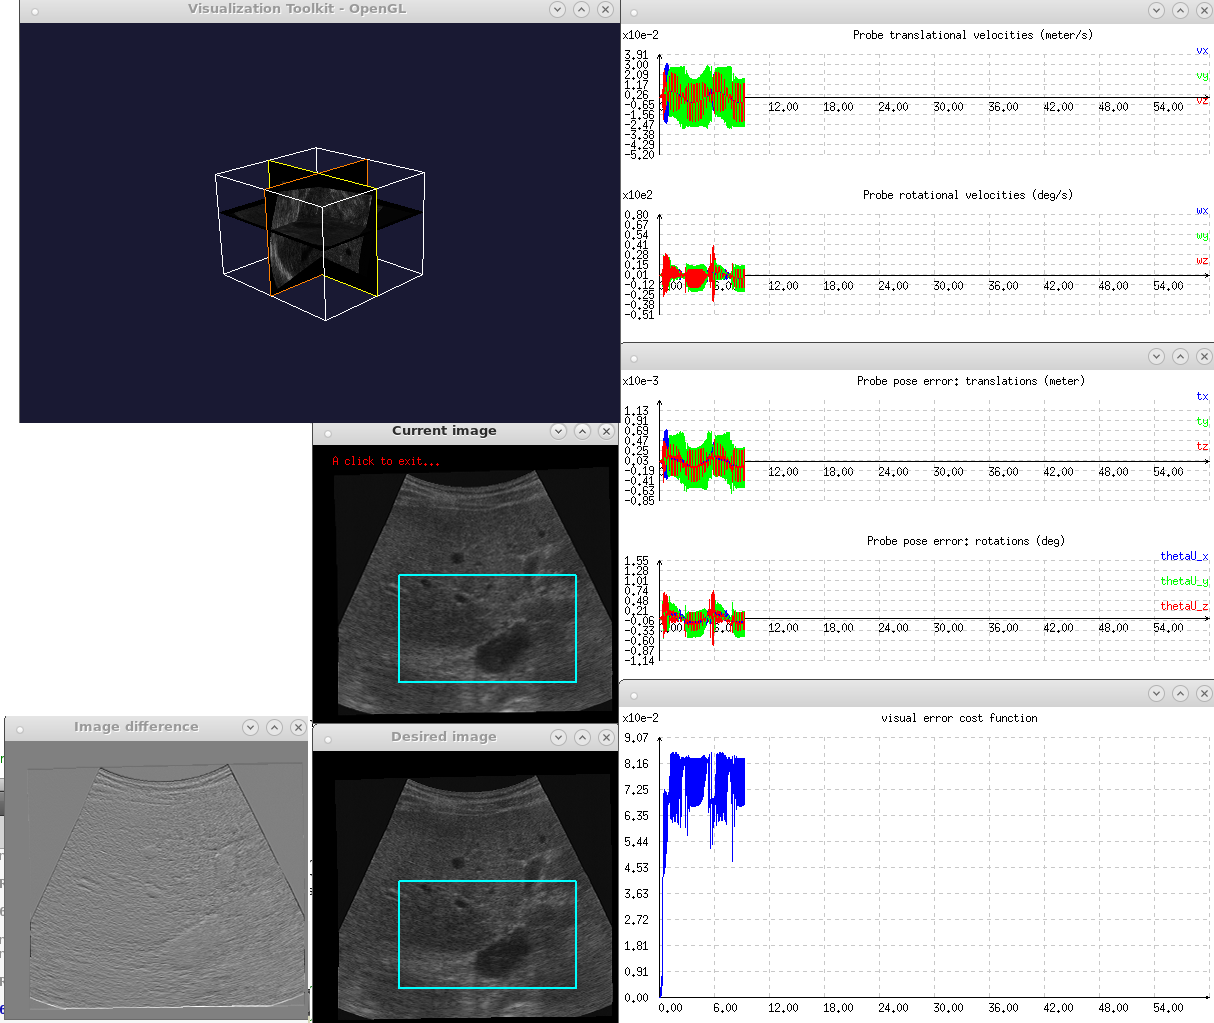
\includegraphics[width=1.0\textwidth]{./images/q10_big.png}
    \caption{Asservissement avec un petit gain (lambda=0.8)}
    \label{bigGain}
\end{figure}

\subsection{Question 11}
%TODO
\begin{figure}[H]
    \centering
    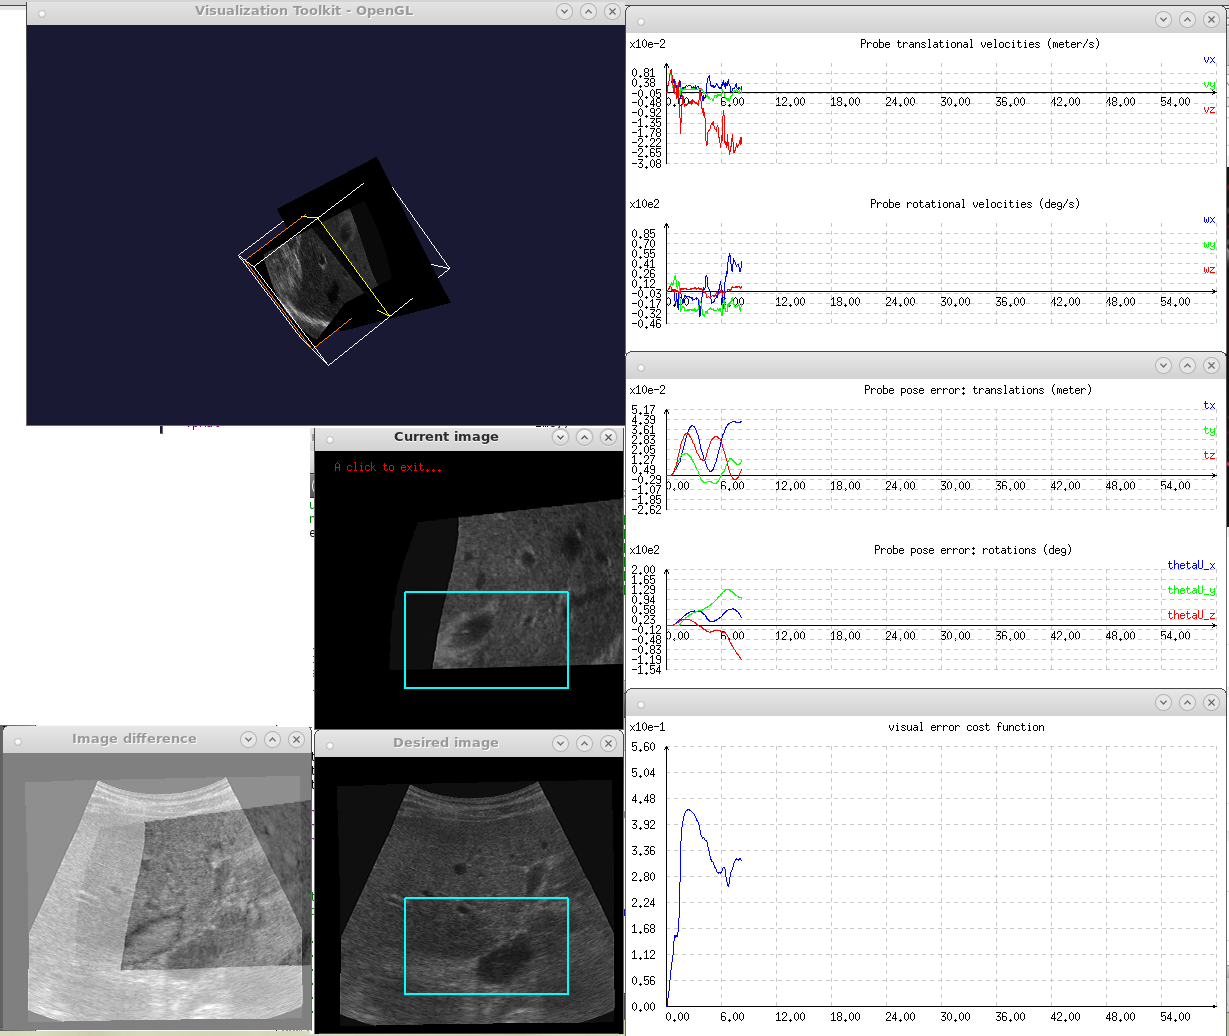
\includegraphics[width=1.0\textwidth]{./images/q11_0,4.png}
    \caption{Asservissement avec mouvement rapide }
    \label{fastMove}
\end{figure}

\subsection{Question 12}
%TODO Expliquer le but de la question
\begin{verbatim}
%Mettre le code ici
\end{verbatim}
%TODO Commenter le code 

\subsection{Question 13}
%TODO

\section{Conclusion}
%TODO

\end{document}
\grid
\grid
